\subsection{Implementation of Gatys style transfer}
As a part of our project we have implemented a video version of the traditional style transfer proposed in Gatys \cite{Gatys:1}, where each frame is individually generated in the way described here and put together as a new video.\newline\newline
This was the first style transfer method we implemented, as it is the most well known method and also one of the simplest. Gatys style transfer is also the basis for many other research papers and is often referenced and used to compare results with. This includes the research papers we have discussed in the Related Works Section. Our implementation also serves as the basis for our later implementations of Ruder \cite{Ruder:1} and Huang \cite{Huang:1} style transfer.  \newline\newline
The main method in which we generate our images is that we have two loss functions with separate weights. One loss function is for style loss and the other one is for content loss, where we use Gram Matrices to calculate the distances for the loss of style. Then we train our model to minimize the loss. All this is explained more in depth in Section \ref{sec:gatys}.\newline\newline
As described earlier, for Gatys implementation we run the style-image, content image and our generated image through the pre-trained VGG-19 network and extract pre-selected layers for content and style. In our implementation we use \textit{conv5.2} for content. For style we use 5 layers in the network: \textit{conv1.1, conv2.1, conv3.1, conv4.1 and conv5.1}.\newline\newline
The original implementation of Gatys style transfer is made primarily to be used for style transfer on single images. However, in our implementation we are making video style transfer. To do this we created a method to split a video into a list of all the single images in a video, with a frame rate chosen by us. Then we can use the Gatys style transfer on the images on by one, and at the end put them back together to a video.\newline\newline
As Gatys style transfer is primarily made for image style transfer, some problems arise when we try to implement it in video form. When we train each frame in the video separate from each other, the randomness in the training will create some difference in the styling between adjacent frames. That means two frames which are almost identical might end up being quite different when styled. This causes the video to have a lot of noise and movement. In some cases this produces a very nice effect and can actually look better than other more advanced implementations. But in other cases it would be preferable to have less noise.
\begin{figure}[!ht]
\begin{center}
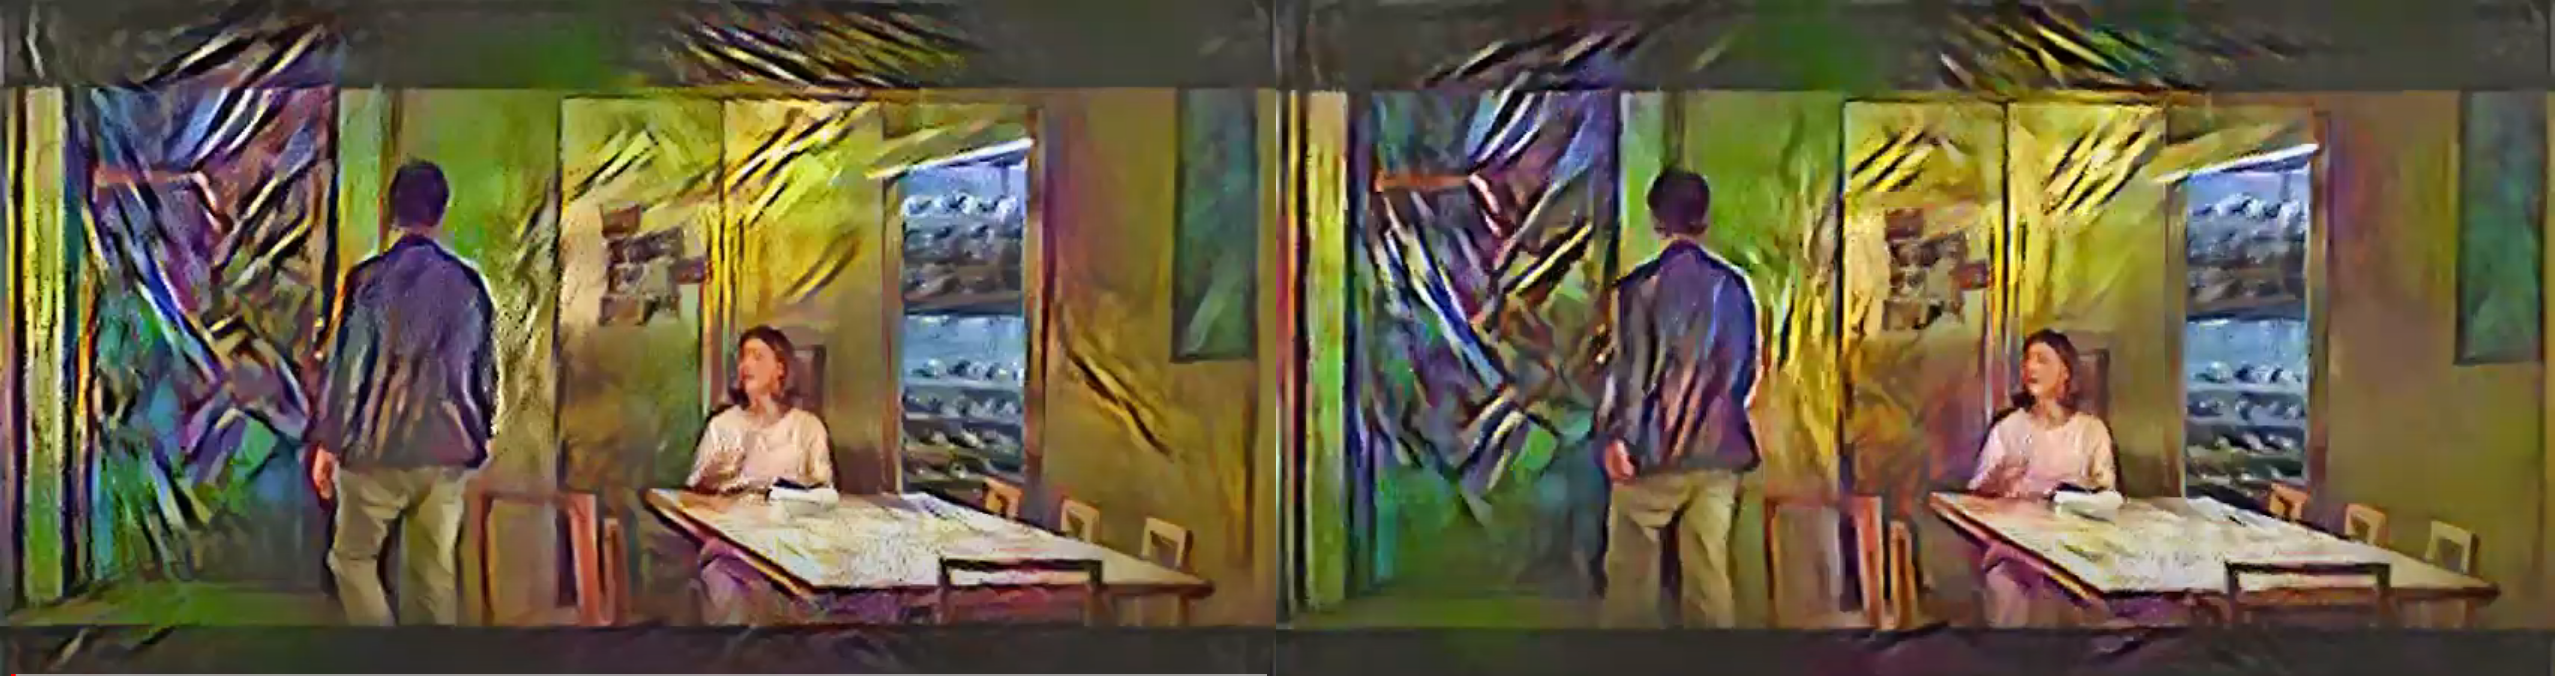
\includegraphics[scale=0.15]{report/Method/images/gatys_adjacent.png}
\caption{Two consecutive frames produced with Gatys style transfer with the La Muse (Picasso) as style reference}
\label{fig:Adjacent frames with ruder}
\end{center}
\end{figure}\newline\newline
In Figure \ref{fig:Adjacent frames with ruder}, we have two adjacent frames which show the randomness that appears. On the wall to the right there is some styling effect on the first frame, which does not appear in the next frame.\newline\newline
This leads us to our next implementation, which is based on the paper of Ruder \textit{et al.} \cite{Ruder:1}. In this implementation we try to improve the video style transfer we implemented from Gatys by introducing a temporal component to the loss function.